\section{Methodology}

\subsection{Model}

We assume an application model that is similar to Secret~\cite{secret}.
\begin{figure}
\centering
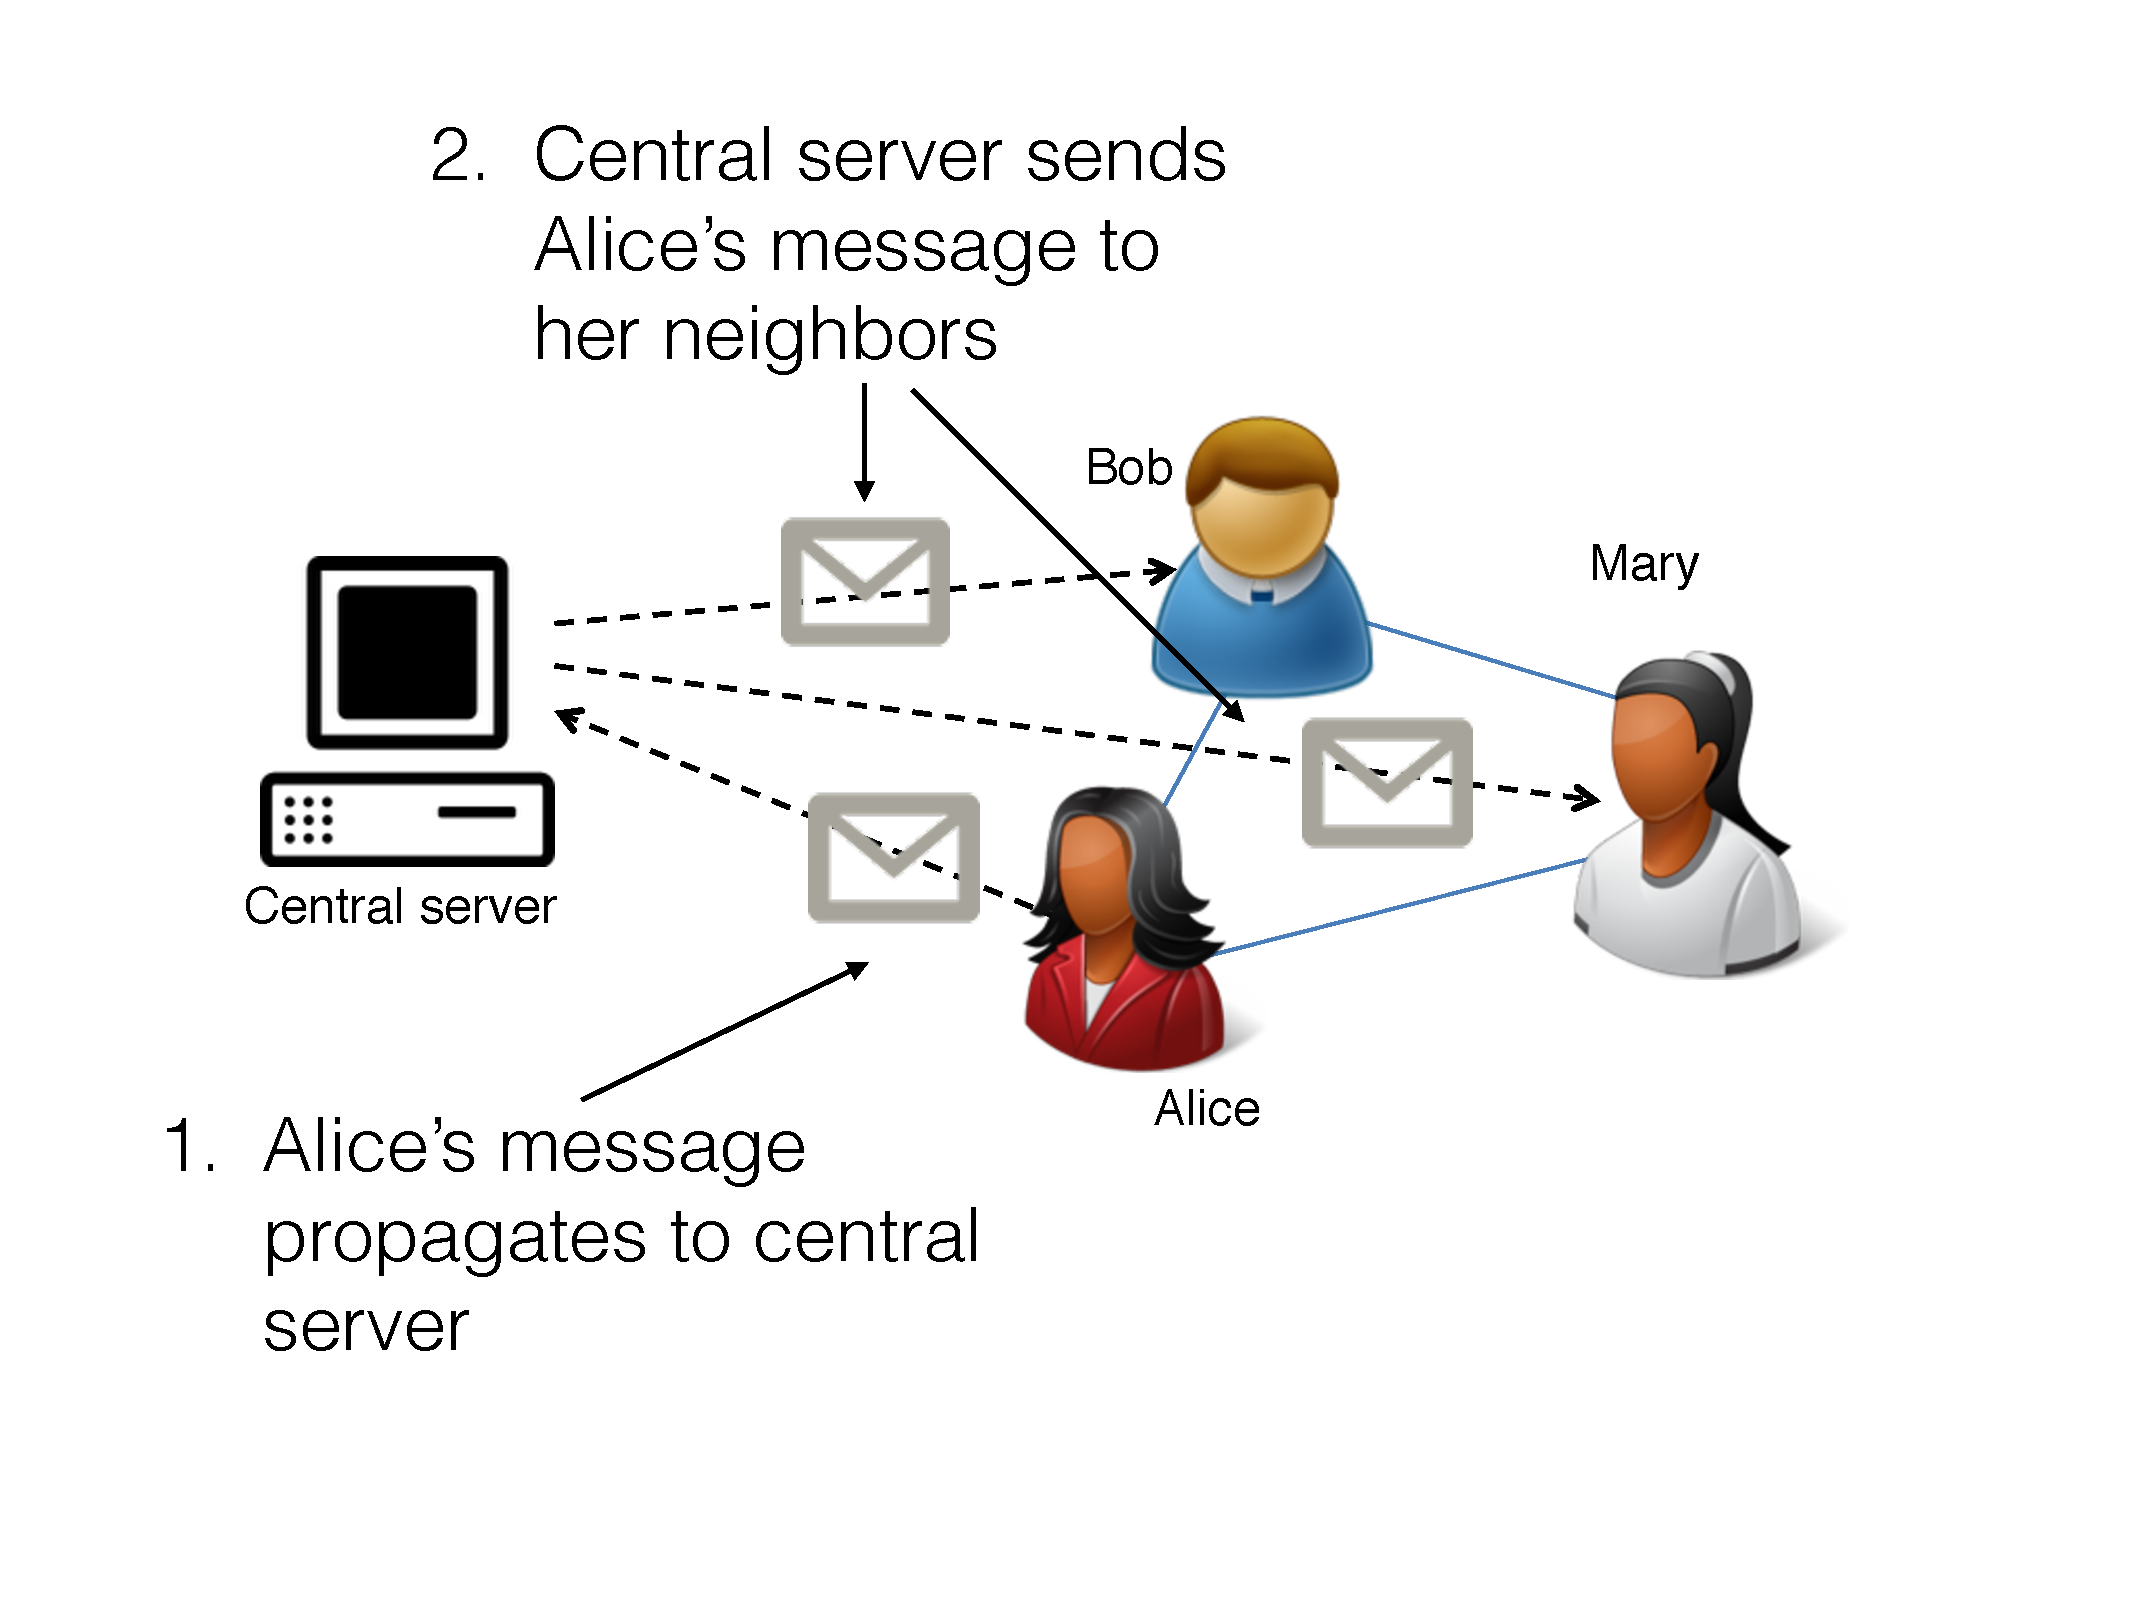
\includegraphics[height = 2.4in]{figures/secret_infrastructure}
\caption{An overview of the infrastructure for a typical anonymous social network.}
\label{fig:secret_infrastructure}
\end{figure}
Fig.~\ref{fig:secret_infrastructure} shows how a typical anonymous microblogging network works. Users are connected to friends as in a regular social network; we model this social network as a graph $\mathcal G(V,E)$, where $V$ denotes the set of vertices, or participants, in the network, and $E$ denotes the set of edges. When a source node, Alice, decides to send a message to her friends, her message is routed to a centralized server first. We denote the source node by $v^*$. The server propagates the message to Alice's neighbors, $\mathcal N(v^*)$. Alice's neighbors do not know who sent or authored the message. %To them, the message is from the centralized server instead of directly from Alice, and does not have any information about the sender herself. 
If one of Alice's friends decides to ``like'' the message, the message will be further propagated to her friend's friends. Thus, whenever a user receives a message, he/she does not know if a neighboring friend sent it, or if it was simply liked by a friend. We assume that propagation occurs with some time delay, which captures the time between the server pushing a message and the receipient actually seeing it. We model the delay between a user $i$ liking a message and the user's friend $j$ seeing the message as a random variable $\theta_{ij}$; the $\theta_{ij}$'s, or delays across each edge in the social graph, are assumed to be iid random variables. We do not specify the distribution of $\theta_{ij}$ \emph{a priori}; in principle, this should be informed by measurements of real social network usage.

We assume there are $K$ spies in the network, $o_1,\ldots,o_K$. Each spy $o_i$ will collect the timestamp $t_i$ at which it first receives the message.

Our adversarial model derives directly from the normal model. A moderately powerful adversary is able to compromise certain users in the social network. This may be accomplished by offering some incentives to users and recruit them act as spies. The spies are not active, but are instead passive observers. The only thing that differentiates spies from honest users is that spies will collect all messages, and then send these messages to the adversary periodically. The adversary uses the collected messages to attempt to track down the perpetrator of the message. Therefore, the 

The central adversary will receive different sets of messages, and it will need to group them into a \emph{collection} -- a group of messages received at different nodes that came from the same source. We assume that these messages are not encrypted, and thus the adversary can use the plaintext information directly to identify the correct collection membership. 

\subsection{Efficacy of deanonymization}

A number of factors could impact the efficacy of deanonymization:

\begin{description}
\item[Underlying graph structure] The underlying graph structure may affect deanonymization a lot. For example, a tree-like structure with no loops is easier to deanonymize because there are fewer possible paths to analyze. In our simulation, we study many different types of graphs, including trees, Erdos-Renyi, and Barabasi-Albert graphs.
\item[Fraction of spies] The fraction of spies will greatly impact the deanonymization performance. Fewer spies means less information, and thus makes the true source much harder to track. Using simulation, we want to \emph{quantify} how many spies are needed to efficiently find the true source.
\item[Location of spies] We hypothesize that uniform distribution of spy nodes will be most effective in deanonymizing nodes, because they are able to intercept messages on a wide scale. 
\item[Propagation latency] The propagation latency is modeled as the time for the message to leave one user and is seen by another user. 
We model the propagation latency in two ways: using a Gaussian distribution, and a geometric random variable. 
\item[Estimator] We try different methods of estimation. The majority of our effort is spent on adapting the observer model~\cite{pinto} to our spy nodes setting.
\end{description}

\subsection{Estimators}
Initially, we attempted to come up with some estimators on our own. \todo{Should we mention the Jordan estimators here?}

The observer model estimator~\cite{pinto} is a maximum likelihood estimator. The setup is quite similar to our simulation: given a graph $G$, there exists a set of $K_a$ observers that pick up information transmitted in the network. The collected information has receiving timestamp, as well as the direction information (e.g. observer $o$ receives the message from neighbor $v$). Before diving into the actual estimator equations, we need to define some terms:

Let $\boldsymbol{d}$ be the timestamp differences of observed arrivals with respect to some reference spy node, and defined as

\begin{equation}
  \boldsymbol{d}_k = t_{k} - t_1
\end{equation}

where $t_i$ indicates the observed message receiving timestamp at observer $i$, and $k$ = 1 ... $K_a$.

The next term is the determinstic delay, which is the delay that one \emph{should} observe if the information propagated from some source $s$ ($s$ is an honest node in the graph):

\begin{equation}
  \boldsymbol{\mu}_{s,k} = \mu (|P(s, o_{k+1})| - |P(s, o_1)|)
\end{equation}

where $|P(u, v)|$ denotes the number of edges on the path that connects nodes $u$ and $v$. 

\begin{equation}
  \boldsymbol{\Lambda}_{k, i} = \begin{cases}
    |P(o_1, o_{k+1})| & \text{if $k = i$} \\
    |P(o_1, o_{k+1}) \cap P(o_1, o_{i+1})| & \text{if $k \neq i$}.
  \end{cases}
\end{equation}


The authors present a source estimator equation for general trees:

\begin{equation}
\label{eq:general}
\hat{s} = \arg\max_{s \in \tau_{a}} \dfrac{\exp(-\frac{1}{2} (\boldsymbol{d} - \boldsymbol{\mu}_{s})^{T} \boldsymbol{\Lambda}_s^{-1} (\boldsymbol{d} - \boldsymbol{\mu}_s) }{|\boldsymbol{\Lambda}_s|^{1/2}}.
\end{equation}

Equation \ref{eq:general} can be applied to general graphs, However, if the underlying graph is tree-structured, equation \ref{eq:general} simplifies to

\begin{equation}
\label{eq:tree}
\hat{s} = \arg\max_{s \in \tau_{a}} \boldsymbol{\mu}_{s}^{T} \boldsymbol{\Lambda}_s^{-1} (\boldsymbol{d} - \frac{1}{2}\boldsymbol{\mu}_s).
\end{equation}
